\section{Описание использованного алгоритма}

\subsection{Основной алгоритм программы}
\begin{figure}[H]
  \centering
  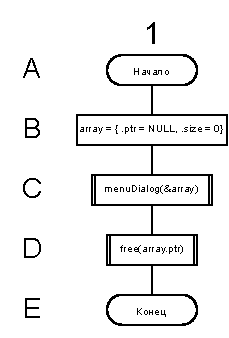
\includegraphics[width=0.35\textwidth]{fun_main}
  \caption{Блок-схема алгоритма работы функции \texttt{main()}}
\end{figure}

\begin{figure}[H]
  \centering
  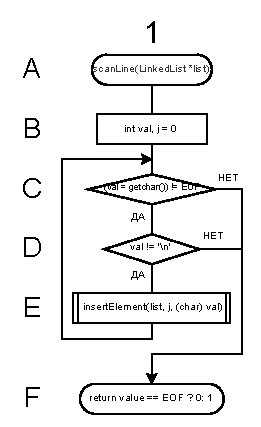
\includegraphics[width=0.4\textwidth]{fun_scanLine}
  \caption{Блок-схема алгоритма работы функции \texttt{scanLine()}}
\end{figure}

\subsection{Описание алгоритма работы со спиками}
\begin{figure}[H]
  \centering
  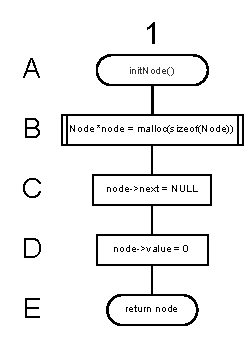
\includegraphics[width=0.3\textwidth]{fun_initNode}
  \caption{Блок-схема алгоритма работы функции \texttt{initNode()}}
\end{figure}

\begin{figure}[H]
  \centering
  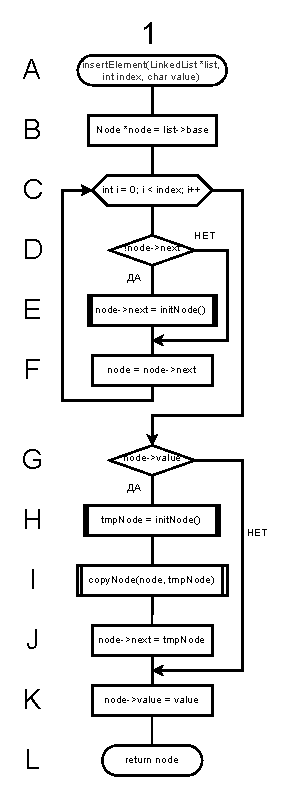
\includegraphics[width=0.45\textwidth]{fun_insertElement}
  \caption{Блок-схема алгоритма работы функции \texttt{insertElement()}}
\end{figure}

\begin{figure}[H]
  \centering
  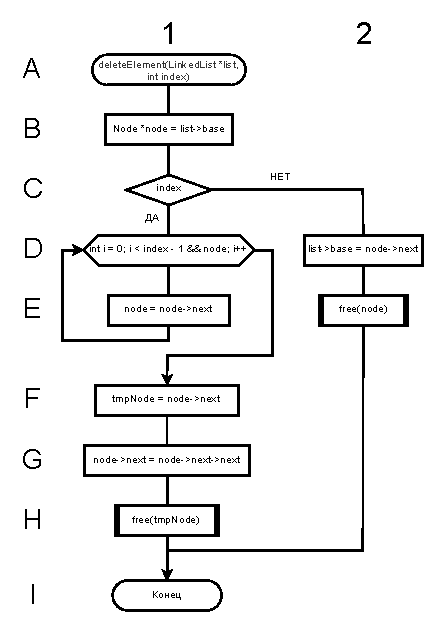
\includegraphics[width=0.5\textwidth]{fun_deleteElement}
  \caption{Блок-схема алгоритма работы функции \texttt{deleteElement()}}
\end{figure}

\begin{figure}[H]
  \centering
  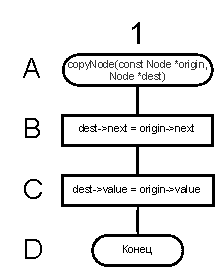
\includegraphics[width=0.275\textwidth]{fun_copyNode}
  \caption{Блок-схема алгоритма работы функции \texttt{copyNode()}}
\end{figure}

\begin{figure}[H]
  \centering
  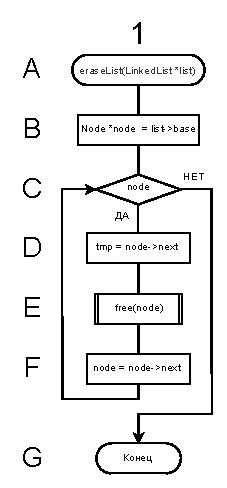
\includegraphics[width=0.275\textwidth]{fun_eraseList}
  \caption{Блок-схема алгоритма работы функции \texttt{eraseList()}}
\end{figure}

\begin{figure}[H]
  \centering
  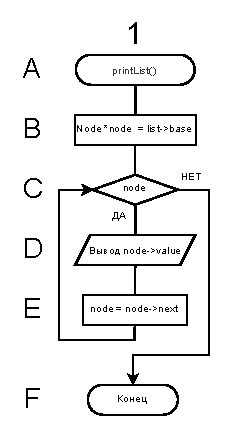
\includegraphics[width=0.275\textwidth]{fun_printList}
  \caption{Блок-схема алгоритма работы функции \texttt{printList()}}
\end{figure}

\subsection{Описание алгоритма обработки списка}
\begin{figure}[H]
  \centering
  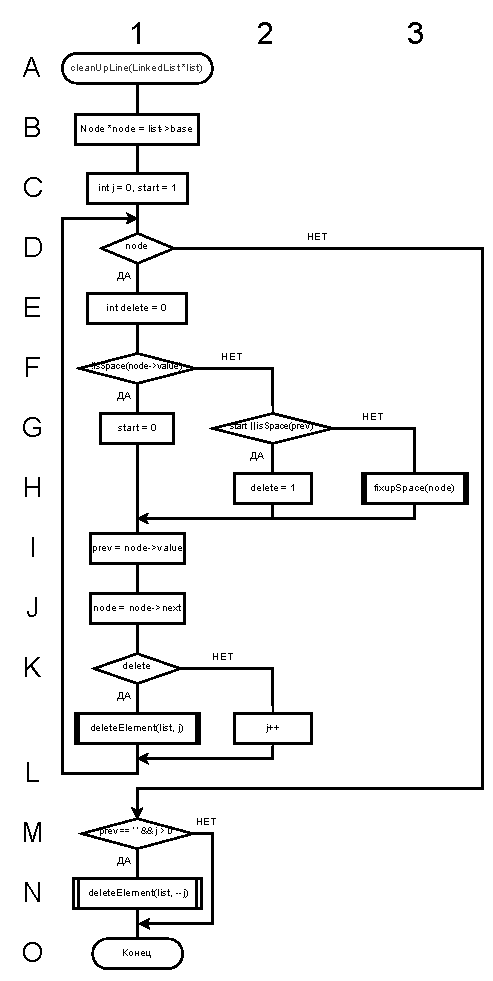
\includegraphics[width=0.6\textwidth]{fun_cleanUpLine}
  \caption{Блок-схема алгоритма работы функции \texttt{cleanUpLine()}}
\end{figure}

\begin{figure}[H]
  \centering
  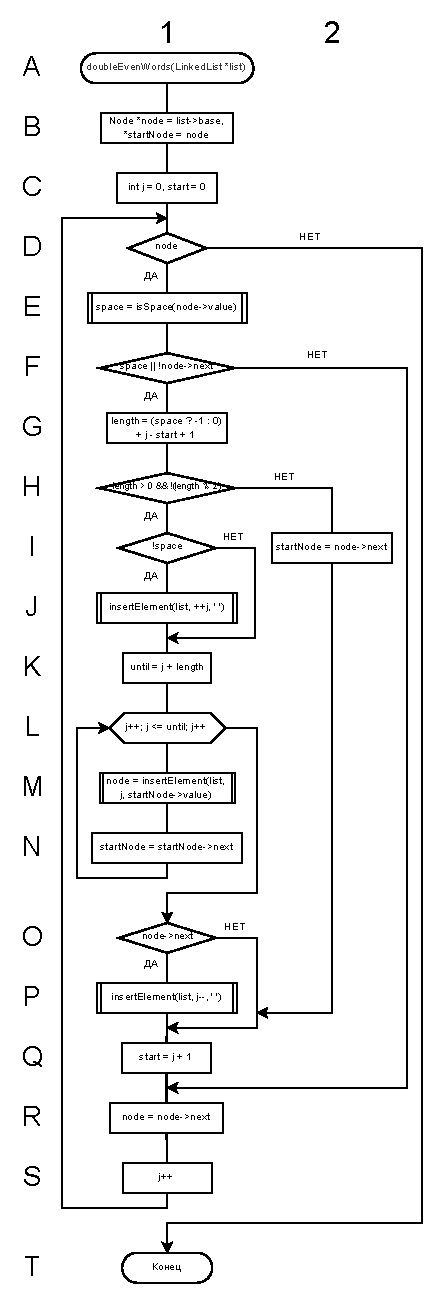
\includegraphics[width=0.46\textwidth]{fun_doubleEvenWords}
  \caption{Блок-схема алгоритма работы функции \texttt{doubleEvenWords()}}
\end{figure}

\begin{figure}[H]
  \centering
  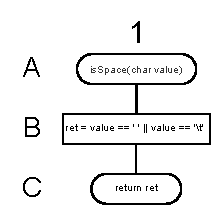
\includegraphics[width=0.275\textwidth]{fun_isSpace}
  \caption{Блок-схема алгоритма работы функции \texttt{isSpace()}}
\end{figure}

\begin{figure}[H]
  \centering
  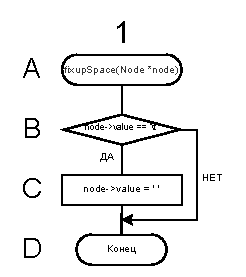
\includegraphics[width=0.3\textwidth]{fun_fixupSpace}
  \caption{Блок-схема алгоритма работы функции \texttt{fixupSpace()}}
\end{figure}